% !TeX encoding = UTF-8
%
% Grafische Oberflächen:
%


%
% Grafische Oberflächen starten auf eigener Seite.
%
\clearpage


\section{Grafische Oberfl{"a}chen}
\label{NU:GO}

\paragraph*{\underline{Pflicht:}}

\begin{ids}{\gls{PGO}}

	\id[0010] Ein Hauptmenü mit Auswahl zum \glqq challenge\grqq~Modus und zum \glqq creative\grqq~Modus.
	
	\id[0020] Ein Menü für der \glqq creativ\grqq~Modus um sich zwischen dem erstellen eines neuen Knotens, einer neuen Herausforderung und dem Laden eines Knotens zu entscheiden.
	
	\id[0030] Ein Menü in dem man sich aussuchen kann, welcher Knoten geladen werden soll.
	
	\id[0040] Ein Menü in dem man eine neue Herausforderung zusammenstellt.
	
	\id[0050] Ein Menü in dem man eine Herausforderung zu spielen auswählen kann.
	
	\id[1010] Ein Editor, in dem man den Knoten bearbeitet.
	
	\id[1020] Im Editor /PGO\_1010/ eine Spielfläche in dem man den Knoten sieht und bearbeitet.
	
	\id[1030] Im Editor /PGO\_1010/ ein Pausenmenü, in dem man im \glqq creative" Modus speichern und in jedem Modus das bearbeiten beenden kann.
	
	\id[1040] Im Editor /PGO\_1010/ ein Zugang um ins Pausenmenü /PGO\_1030/ zu gelangen.

\end{ids}




\paragraph*{\underline{Optional:}}

\begin{ids}{\gls{OGO}}

	\id[0010] Im Hauptmenü /PGO\_0010/ eine Auswahl um die \gls{fa:Credits} anzuzeigen.
	
	\id[0020] Ein Menü für verschiedene Spieleinstellungen.
	
	\id[0030] Im Hauptmenü /PGO\_0010/ eine Auswahl um zum Menü für Spieleinstellungen /OGO\_0020/ zu kommen.
	
	\id[0040] Im \gls{fa:EinstM} /OGO\_0020/ ein Untermenü für die Tastaturbelegung.
	
	\id[0050] Im Einstellungsmenü /OGO\_0020/ ein Untermenü für grafische Einstellungen.
	
	\id[0060] Im Einstellungsmenü /OGO\_0020/ ein Untermenü für audio Einstellungen.
	
	\id[0070] Im Einstellungsmenü /OGO\_0020/ ein Untermenü für eine personaliesierte Farbpalette.
	
	\id[1010] Im Pausenmenü /PGO\_1030/ ein Eintrag um das Einstellungsmenü /OGO\_0020/ anzuzeigen.
	
	\id[1020] Ein Menü für verschiedene Render- und Exportfunktionen.
	
	\id[1030] Im Editor /PGO\_1010/ eine Möglichkeit das Rendermenü /OGO\_1020/ aufzurufen.
	
	\id[1040] /OGO\_1030/ ist nur im \glqq crative\grqq~ Modus und nach bestandener Herausforderung zugänglich.
	
\end{ids}


% ToDo: An sich wäre noch eine direkte Verlinkung auf die Grafiken an der entsprechenden Stelle gut.

%
%
%
\clearpage



%
%
%



\section*{Visualisierungen}








\section{Interaktionsverlauf}

	\begin{description}
		\item[main menu] /PGO\_0010/ Erste Ansicht nach dem starten des Spiels.
		\item[creative] /PGO\_0020/ Untermenü um die Entscheidungsmöglichkeiten für den "creative"-Modus anzuzeigen
		\item[challenge] /PGO\_0050/ Listet alle vorhandenen Herausforderungen auf.
		\item[new challenge] Eintrag um eine neue Herausforderung zu erstellen.
		\item[challenge settings] /PGO\_0040/ Lässt einen alle Einstellungen zu einer neuen Herausforderung einstellen.
		\item[new knot] Spiel startet mit einem minimalem Knoten.
		\item[load] /PGO\_0030/ Listet alle gespeicherten Knoten auf und lässt den Spieler einen auswählen und zum bearbeiten laden.
		\item[in game] /PGO\_1010/ Der Editor in dem Das eigentliche Spiel stattfindet.
		\item[credits] /OGO\_0010/ Anzeige der Mitwirkenden.
		\item[settings] /OGO\_0020/ Einstellungsmöglichkeiten für Audio, Video, Steuerung und Farbpalette.
		\item[save] Speichert das laufende Spiel.
		\item[quit] Beendet das laufende Spiel.
		\item[render options] Bietet dem Nutzer verschiedene Möglichkeiten seinen Knoten zu rändern und zu exportieren.
	\end{description}
   
   ~\\
    
	\begin{figure}[h]
		\centering
	 	\includesvg[svgpath=./, width = 0.95\textwidth]{menu}
	 	\caption{Hauptmenüstruktur beginnend mit /PGO\_0010/. Grau hinterlegtes ist Optional.}
	\end{figure}
	
	%~ \clearpage
	%~ ~\\
	%~ 
	%~ Auch aus dem laufenden Spiel heraus kann der Nutzer die Einstellungen erreichen. Die Menüeinträge in den unterschiedlichen Spielmodi können variieren.
%~ 
	%~ \begin{longtable}{|p{0.25\textwidth}|p{0.75\textwidth}|}
	%~ 
	%~ \hline
	%~ settings & Genau wie aus dem Hauptmenü.\\
	%~ \hline
	%~ save & Speichert den aktuellen Spielstand.\\
	%~ \hline
	%~ quit & Beendet das laufende Spiel. \\
	%~ \hline
	%~ render options & Bietet dem Nutzer verschiedene Möglichkeiten seinen Knoten zu rendern und zu exportieren.\\
	%~ \hline
	%~ 
	%~ \end{longtable}
	
	\begin{figure}[!ht]
		  \centering
		  \includesvg[svgpath=./, width = \textwidth]{ingamemenu}
		  \caption{Zugriffsmöglichkeiten im Editor /PGO\_1010/. Grau hinterlegtes ist Optional.\\\hspace{\textwidth}
			1: Nur im \glqq creative\grqq~ Modus\\\hspace{\textwidth}
			2: Nur im \glqq creative\grqq~ Modus und nach bestandener Herausforderung}
	\end{figure}

	
\clearpage
%~ 
%~ \begin{landscape}
%~ 
	%~ \section{Benutzerinteraktionsmodelle}
%~ 
	%~ \begin{figure}[!h]
		%~ \centering
	 	%~ \includesvg[width = 0.99\textwidth]{menu}
	 	%~ \caption{Hauptmenüstruktur beginnend mit /PGO\_0010/. Grau hinterlegtes ist Optional.}
	%~ \end{figure}
	%~ 
%~ \end{landscape}
%~ 
%~ \clearpage
%~ 
%~ \begin{landscape}
%~ 
	%~ \begin{figure}[h]
		%~ \centering
	 	%~ \includesvg[width = 1.1\textwidth]{ingamemenu}
	 	%~ \caption{Zugriffsmöglichkeiten im Editor /PGO\_1010/. Grau hinterlegtes ist Optional.\\\hspace{\textwidth}
			%~ 1: Nur im \glqq creative\grqq~ Modus\\\hspace{\textwidth}
			%~ 2: Nur im \glqq creative\grqq~ Modus und nach bestandener Herausforderung}
		%~ \label{fig:ingamemenu}
	%~ \end{figure}
	%~ 
%~ \end{landscape}
	%~ 
%~ \clearpage
%~ 
%~ 
%~ 
%
%
%
\section{Grafische Bedienungs-Oberfl{"a}chen (\gls{fa:MockUp}s)}
	
	\begin{figure}[ht]
	  \centering
	  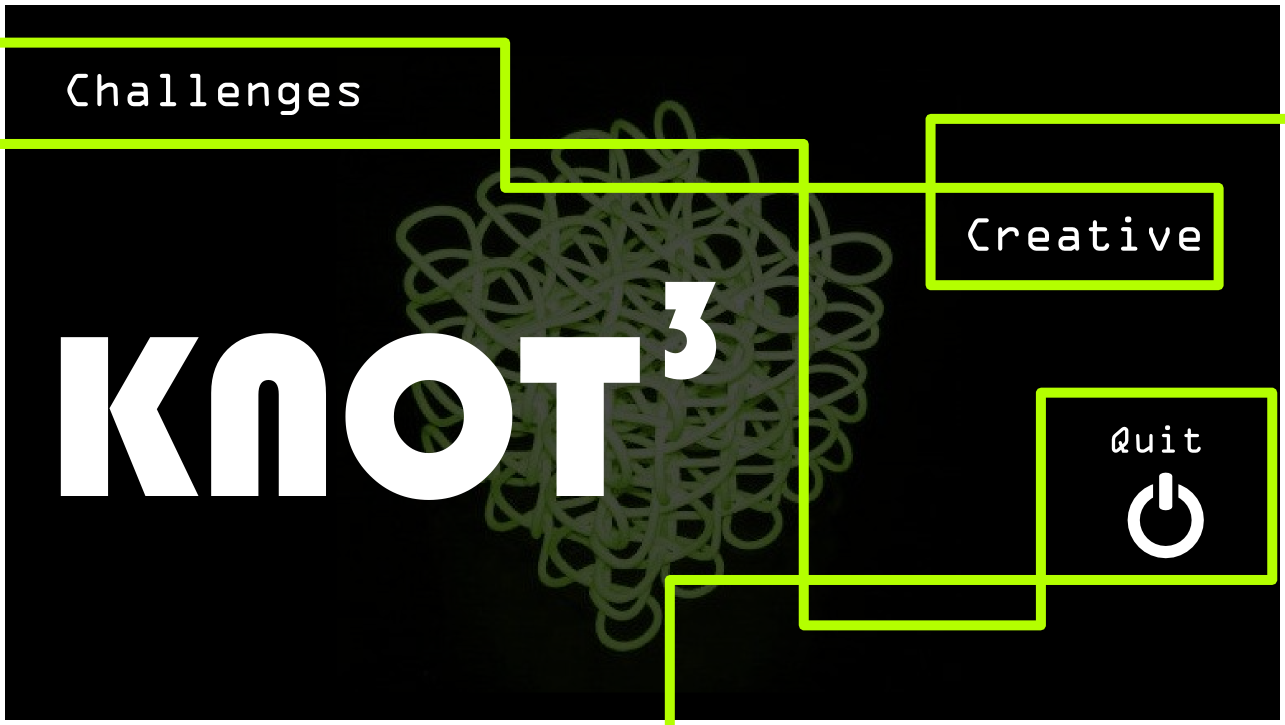
\includegraphics[width = 0.95\textwidth]{Inhalt/Nutzung/Grafiken/Grafische_Oberflaechen/01_Knot3-mainscreen.png}
	  \caption{Mögliches Hauptmenü /PGO\_0010/}
	  \label{fig:mainscreen}
	\end{figure}

	\begin{figure}[!ht]
	  \centering
	  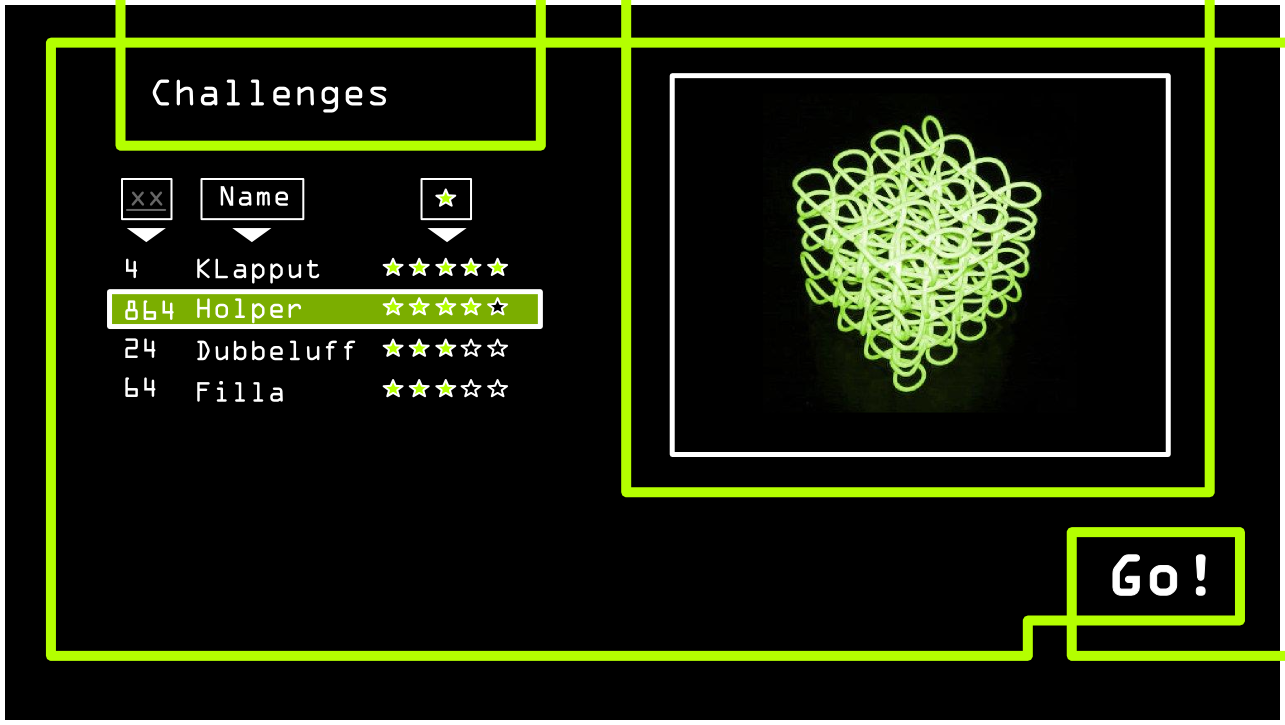
\includegraphics[width = 0.95\textwidth]{Inhalt/Nutzung/Grafiken/Grafische_Oberflaechen/04_Knot3-select-Challenge.png}
	  \caption{Auswahlmenü für die Herausforderungen /PGO\_0050/, mit Ausschnitt der Auswahlliste}
	  \label{fig:selCh}
	\end{figure}
	
	\begin{figure}[ht]
	  \centering
	  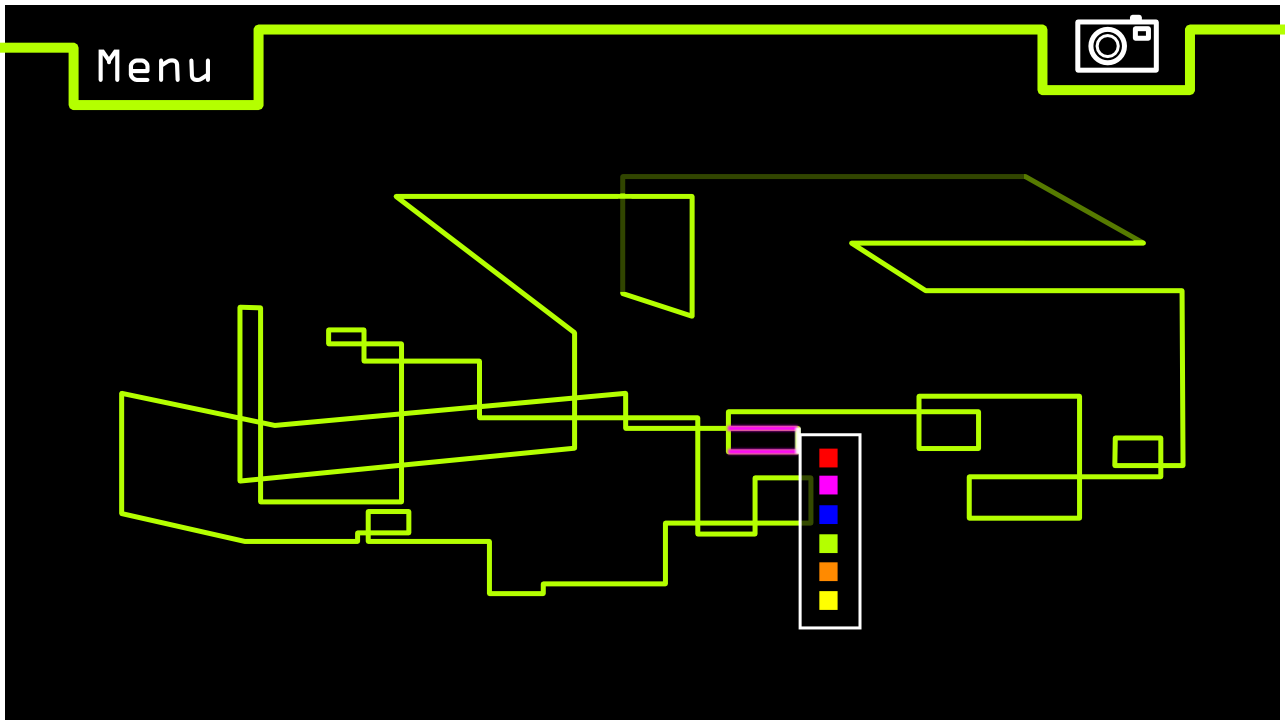
\includegraphics[width = 0.95\textwidth]{Inhalt/Nutzung/Grafiken/Grafische_Oberflaechen/05_Knot3-Colour-select.png}
	  \caption{Editoransicht /PGO\_1010/ mit geöffneter Farbauswahl zum Kanten einfärben /OFA\_200/.}
	  \label{fig:chooseC}
	\end{figure}
	
	\begin{figure}[ht]
	  \centering
	  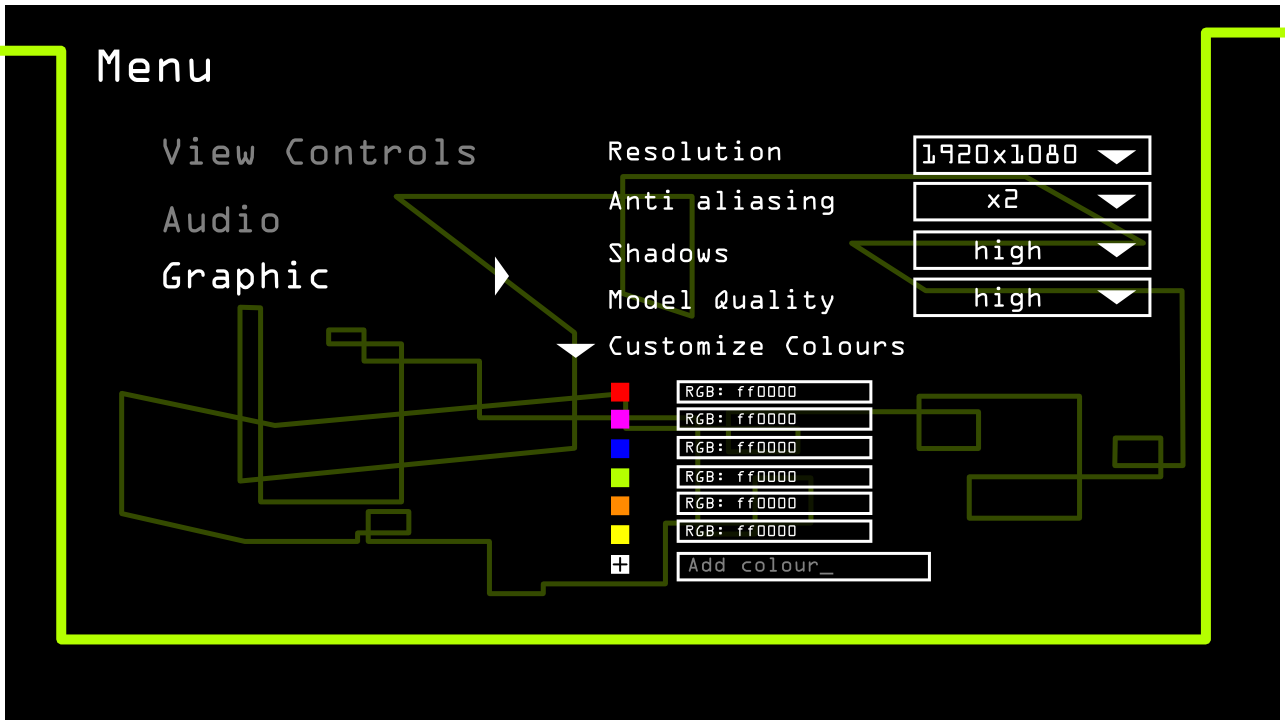
\includegraphics[width = 0.95\textwidth]{Inhalt/Nutzung/Grafiken/Grafische_Oberflaechen/08_Knot3-menu-graphics.png}
	  \caption{Mögliches Einstellungsmenü mit geöffnetem Untermenü für die Grafikeinstellungen. /OGO\_0020/ und /OGO\_0050/}
	  \label{fig:setGFX}
	\end{figure}
	
	\begin{figure}[ht]
	  \centering
	  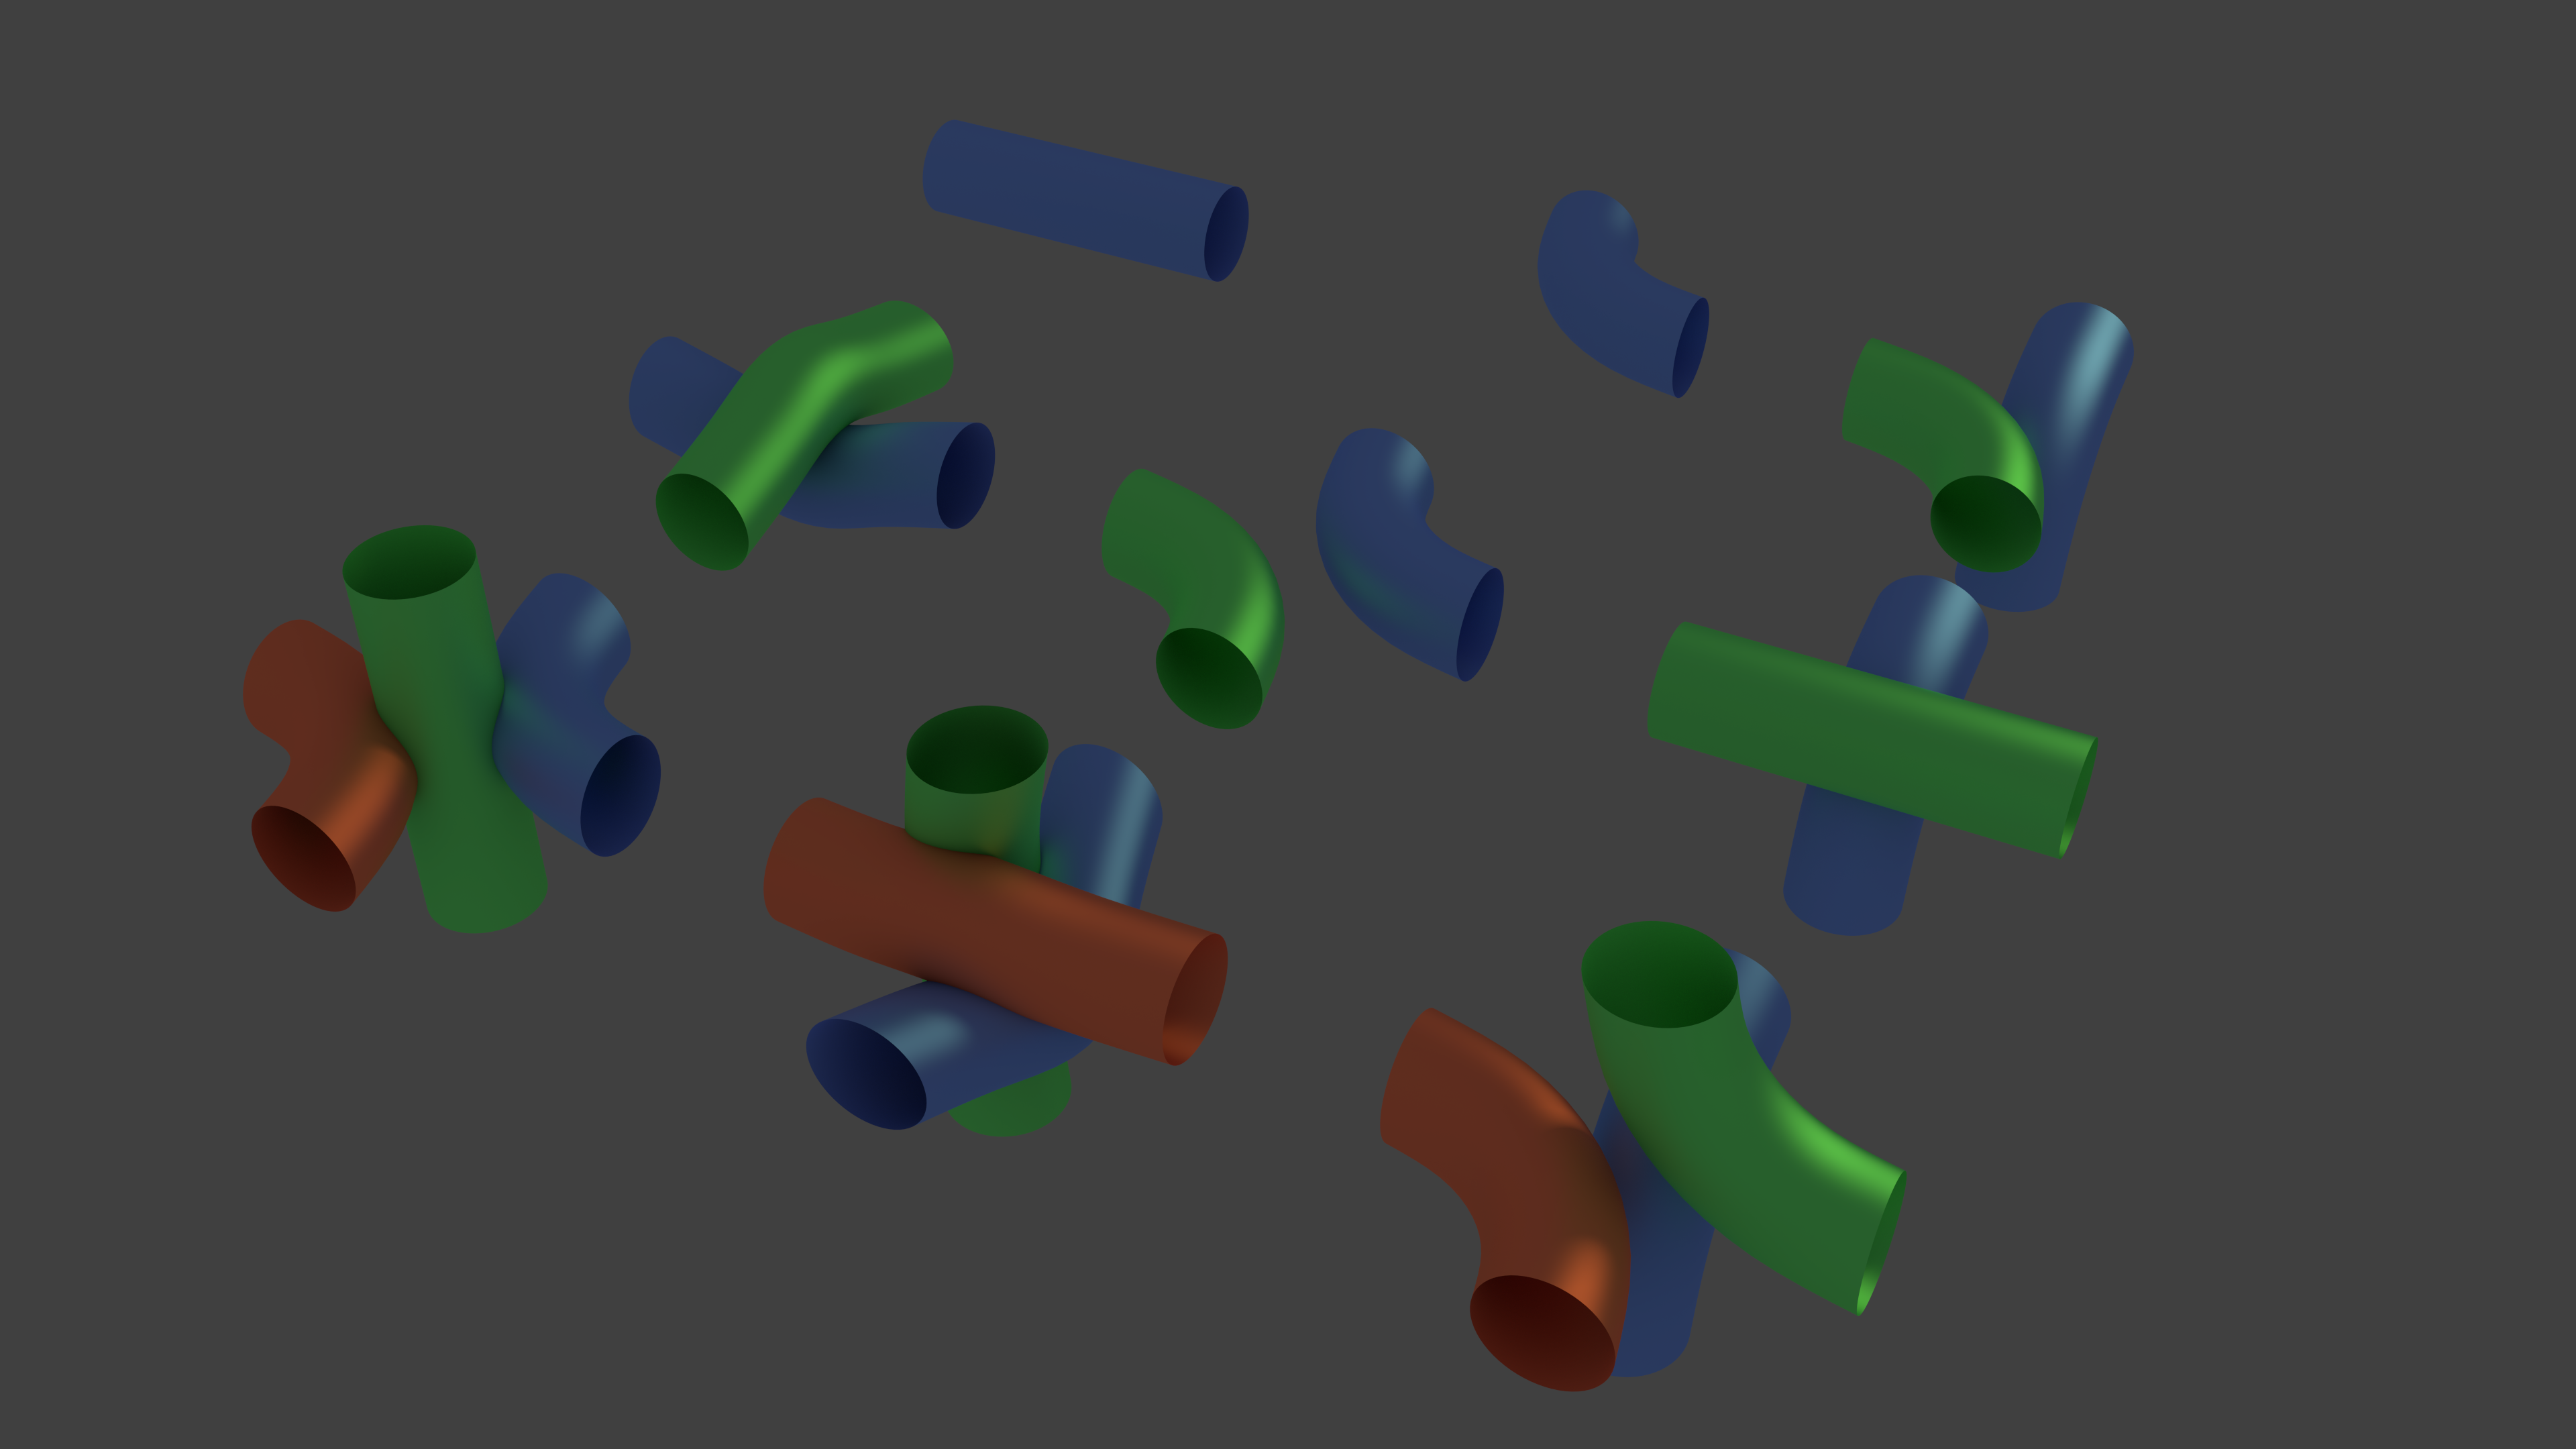
\includegraphics[width = 0.95\textwidth]{Inhalt/Nutzung/Grafiken/Grafische_Oberflaechen/Pipes2.png}
	  \caption{Verschiedene Übergänge für die Kanten}
	  \label{fig:pipes2}
	\end{figure}
	

\clearpage
	


\subsection{Spielz{"u}ge}~\\


\subsubsection{Beispiele g{"u}ltiger Z{"u}ge}


~\\
Grundsätzlich ist jede Transformation, die mit der Spielmechanik machbar ist ein \gls{fa:gZug}.
Die Spielmechanik verhindert das entstehen von doppelt belegten Kanten, was einen ungültigen Zustand darstellen würde.



\subsubsection{Beispiele unm{"o}glicher Z{"u}ge}
	\begin{figure}[htb]
	  \centering
	  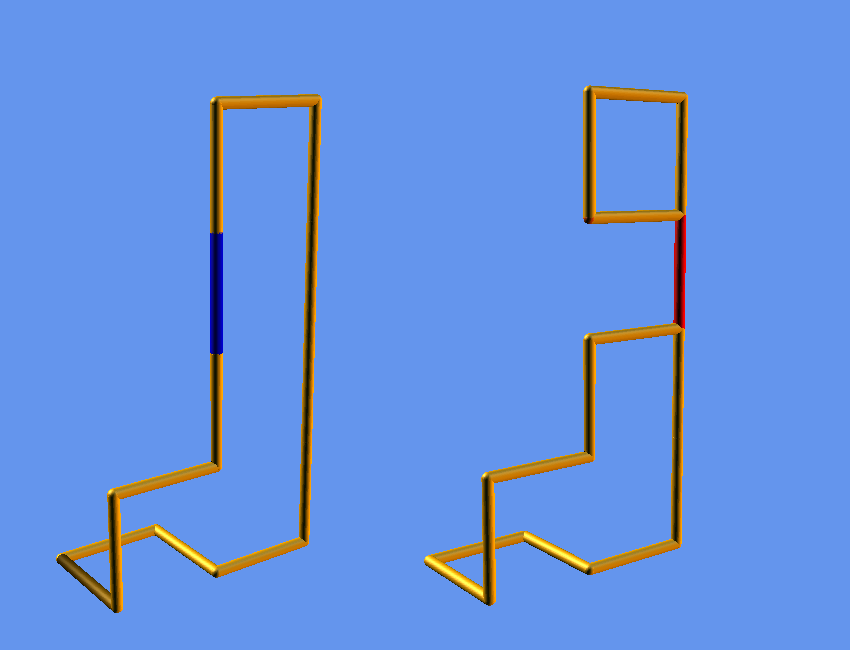
\includegraphics[width = \textwidth]{Inhalt/Nutzung/Grafiken/Grafische_Oberflaechen/Ungueltiger_Zug.png}
	  \caption{Parallele Kantenvereinigung}
	  \label{fig:zug1}
	\end{figure}
Der Knoten auf der linken Seite \ref{fig:zug1} beschreibt eine gültige Spielsituation. Der Spieler wählt eine Kante (blaue Hervorhebung) aus, um einen weiteren \gls{fa:Zug} vorzunehmen.
Einem Spieler ist es nicht möglich, zwei parallele Kanten (hier: die Blaue und die Rote) zu einer Kante zu vereinen. Das ist ein \gls{fa:uZug}. Der Knoten soll immer aus einem geschlossenen Kreis von Kanten bestehen. Der Knoten auf der rechten Seite \ref{fig:zug1} ist daher eine ungültige Spielsituation.

\clearpage

